\section{Siatka karnaugh}

\subsection{Siatki pomocnicze}

\begin{figure}[h!]
    \centering
    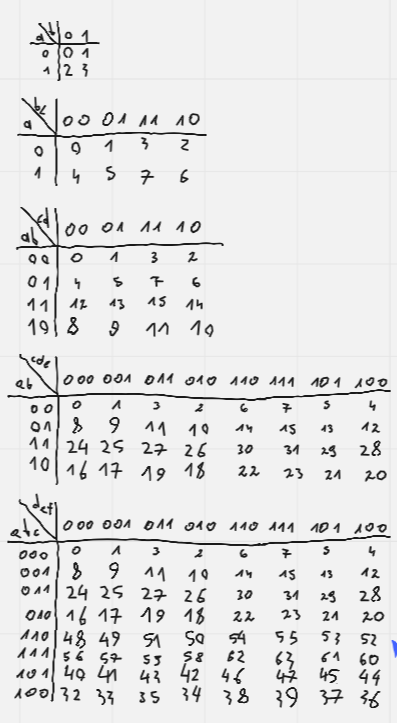
\includegraphics[width=.6\textwidth]{images/karnaugh/k_help.png}
    \caption{duże siatki}
    \label{fig:my_label}
\end{figure}

\newpage

\subsection{Treść zadania}

\begin{figure}[h!]
    \centering
    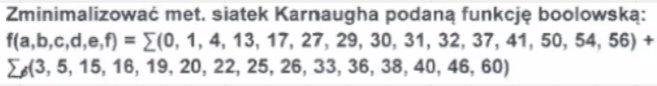
\includegraphics[width=0.6\textwidth]{images/karnaugh/k_ex.png}
    \caption{treść zadania}
    \label{fig:my_label}
\end{figure}

$f(a,b,c,d,e,f)$ - oznacza że układ który tworzymy ma 6 wejść. a - najstarszy bit(msb), f - najmłodszy bit(lsb)

\vspace{1em}

$\sum_m$ - dla tych wartości funkcja przyjmuje wartość ,,1''

\vspace{1em}

$\sum_\phi$ - dla tych wartości funkcja przyjmuje wartość ,,-''

\vspace{1em}

$\Pi$ - dla tych wartości funkcja przyjmuje wartość ,,0''

\subsection{Rozwiązanie}

\subsubsection{Siatka z wartościami liczbowymi}

\begin{figure}[h!]
    \centering
    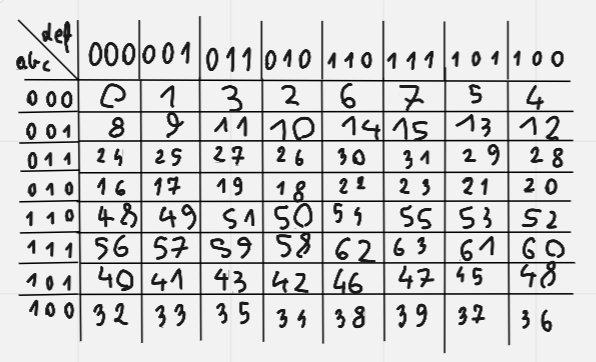
\includegraphics[width=0.45\textwidth]{images/karnaugh/k_t0.png}
    \caption{siatka pomocnicza}
    \label{fig:my_label}
\end{figure}

\subsubsection{Siatka bez połączonych jedynek}

\begin{figure}[h!]
    \centering
    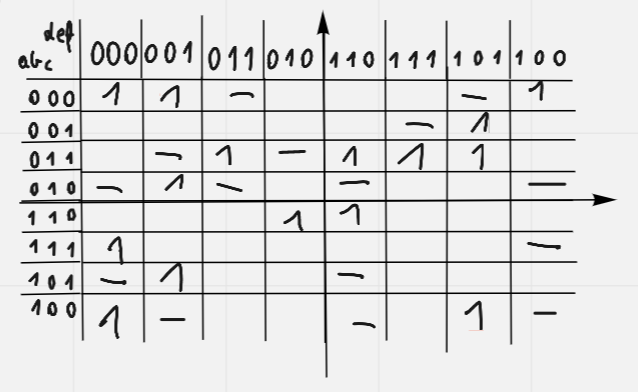
\includegraphics[width=0.45\textwidth]{images/karnaugh/k_t1.png}
    \caption{siatka bez zaznaczonych obszarów}
    \label{fig:my_label}
\end{figure}

\newpage

\subsubsection{Siatka z połączonymi jedynkami}

Obszary, które możemy ująć wspólnie \textbf{muszą być symetryczne względem osi symetrii poziomej i pionowej} - znaczy to tyle, że jeśli "złoży się" siatkę wzdłuż osi symetrii, obszar powinien się pokrywać z jego drugą częścią po przeciwległej stronie (chyba, że cały obszar znajduje się w jednej ćwiartce). Warto nadmienić, że w siatkach o większych wymiarach (3x2 i więcej) każda ćwiartka też ma swoje osie symetrii działające analogicznie do całej siatki. W praktyce tyczy się to tylko siatek o min. 3 zmiennych. W obszarach \textbf{można zawierać jedynki (lub analogicznie zera) i myślniki (stany niedozwolone)}. \textbf{Każdy obszar musi mieć $2^n$ elementów i mieć kształt prostokąta}. Gdy jedynki są na krawędziach siatki, można je połączyć ze sobą (podobnie z narożnikami) przy zachowaniu symetrii, tj. po jednej i drugiej stronie siatki musi znajdować się tyle samo elementów.

\begin{figure}[h!]
    \centering
    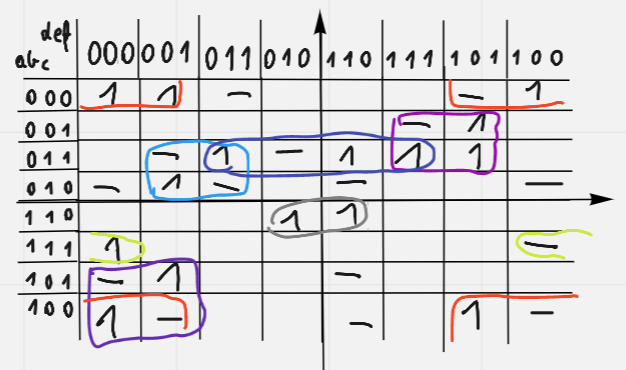
\includegraphics[width=0.6\textwidth]{images/karnaugh/k_t2.png}
    \caption{siatka z zaznaczonymi obszarami}
    \label{fig:my_label}
\end{figure}

\subsubsection{Wynik}

\begin{figure}[h!]
    \centering
    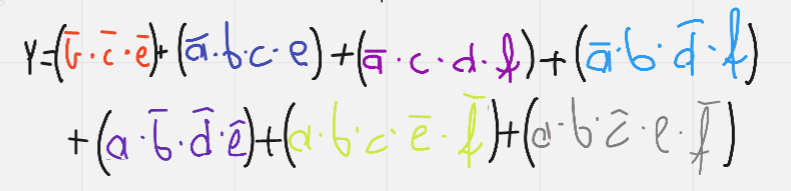
\includegraphics[width=.6\textwidth]{images/karnaugh/k_r.png}
    \caption{ostateczne funkcja}
    \label{fig:my_label}
\end{figure}

\subsection{Klik}

\url{https://www.charlie-coleman.com/experiments/kmap/}